\item Two cells are connected between points A and B as shown. Cell 1 has emf of 12 V and internal resistance of 3$\Omega$. Cell 2 has emf of 6V and internal resistance of 6$\Omega$. An external resistor R of 4$\Omega$ is connected across A and B. The current flowing through R will be \underline{\hspace{2.5cm}} A.
    \begin{center}
        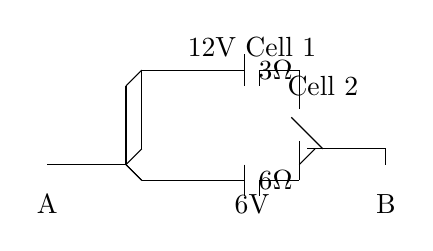
\begin{tikzpicture}
            \draw[-] (0,0) -- (1,0);
            \draw[-] (1,0) -- (1,1);
            \draw[-] (1,1) -- (1.2,1.2);
            \draw[-] (1,0) -- (1.2,-0.2);
            \draw[-] (1.2,1.2) -- (1.2,0.2);
            \draw[-] (1.2,0.2) -- (1,0);
            \draw[-] (1.2,-0.2) -- (1,0);
            \draw (1.2,1.2) -- (2,1.2);
            \draw (1.2,-0.2) -- (2,-0.2);
            
            % Cell 1
            \draw (2,1.2) -- (2.5,1.2);
            \draw (2.5,1.4) -- (2.5,1);
            \draw (2.7,1.2) -- (2.7,1);
            \node at (2.6,1.5) {12V Cell 1};
            \node at (2.9,1.2) {3$\Omega$};
            \draw (2.7,1.2) -- (3.2,1.2);
        
            % Cell 2
            \draw (2,-0.2) -- (2.5,-0.2);
            \draw (2.5,0) -- (2.5,-0.4);
            \draw (2.7,-0.2) -- (2.7,-0.4);
            \node at (2.6,-0.5) {6V};
            \node at (2.9,-0.2) {6$\Omega$};
            \draw (2.7,-0.2) -- (3.2,-0.2);
        
            % Connecting back to B
            \draw (3.2,1.2) -- (3.2,0.7);
            \draw (3.2,0.3) -- (3.2,-0.2);
            \draw (3.4,0.2) -- (3.2,0);
            \draw (3.1,0.6) -- (3.5,0.2);
            \draw (3.3,0.2) -- (4.3,0.2);
            \node at (3.5,1) {Cell 2};
            \draw (4.3,0.2) -- (4.3,0);
            
            % Points A and B
            \node (A) at (0,-0.5) {A};
            \node (B) at (4.3,-0.5) {B};
        \end{tikzpicture}
    \end{center}